% This file does not need to be changed.
% Last edit: 2021-03-09
\documentclass[
		paper=a4,				% DIN A4 format
		titlepage=firstiscover, % different margins for titlepage
        draft=false,			% [final | draft]
        fontsize=12pt,			% size of font [10pt | 11pt | 12pt] 
        twoside,              	% [oneside | twoside]
        headsepline,          	% line under header
        headinclude,          	% Header is counted as part of the text
        abstract=true,			% Shows the heading 'Abstract'
        BCOR=10mm,				% Binding correction
        chapterprefix=true,		% Print 'Chapter x' before chapter name
        %bibliography=numbered	% Chapter number for References
        ]
 {scrreprt}						% document class [scrbook|scrreprt] Koma-Script ‘report’ class
 	% Set the document class and its parameters

%%%% PACKAGES TO INCLUDE
%% Graphics
\usepackage{graphicx}					% Display jpgs, png, bmp, ...
\usepackage{pgfplots}					% Render charts and graphs
\pgfplotsset{width=7cm,compat=1.3}		% Size all charts the same
\usepgfplotslibrary{units}
\usepackage{pgf-pie}					% Pie charts
\usepackage{pgfplotstable}				% Displays numerical tables
\usepackage{tikz}						% Draw on figures
\usepackage{smartdiagram}				% fancy diagrams
%%%%
%%   CHANGE COLOURS AND SHAPE STYLES FOR tikzpicture flowcharts
%%%%

\usetikzlibrary{shapes.geometric, arrows}				% flowcharts
\tikzstyle{startstop} = [rectangle, rounded corners, minimum width=3cm, minimum height=1cm,text centered, draw=black, fill=red!30]
\tikzstyle{io} = [trapezium, trapezium left angle=70, trapezium right angle=110, minimum width=3cm, minimum height=1cm, text centered, draw=black, fill=blue!30]
\tikzstyle{process} = [rectangle, minimum width=3cm, minimum height=1cm, text centered, draw=black, fill=orange!30]
\tikzstyle{decision} = [diamond, minimum width=3cm, minimum height=1cm, text centered, draw=black, fill=green!30]
\tikzstyle{arrow} = [thick,->,>=stealth]
				% specify diagram style 
\usepackage{pgfgantt}					% Gantt charts
%% Citations and references - for details: Styles/NDUcitation.info
\usepackage[numbers]{natbib}	% numerical citations
\bibliographystyle{IEEEtranN}	% IEEE-style
\renewcommand{\bibname}{References}  % Rename 'Bibliography' to 'References'
%% Font
\usepackage[UTF8]{inputenc}	% to print accented letters
\usepackage[T1]{fontenc}	% to type accented letters into the tex-files
\usepackage{lmodern}		% To avoid bitmap fonts caused by previous lines
%% Style in general
\usepackage{scrlayer-scrpage}			% Page style
\usepackage[hyphens]{url}				% Nice url in references
\usepackage[hidelinks]{hyperref}		% Clickable references (TOC, table, pic, formular)
\usepackage[acronym,nomain,nonumberlist]{glossaries} 	% To list acronyms
%\usepackage[allcolors=blue]{hyperref}					% All links in blue
%\usepackage[ocgcolorlinks]{ocgx2}						% All links printed black | NOT WORKING YET!
\usepackage{enumitem}									% Enumeration style change
\setlist[itemize]{noitemsep, topsep=0pt}				% No spacing at item lists
\usepackage{lipsum}										% Create dummy text
\usepackage[onehalfspacing]{setspace}					% Set space between each line

%% For debugging
%\usepackage{showframe}						% Shows the margins
%\listfiles									% List the files used and their version numbers in the log file

%%%% USER DEFINED MACROS
%%%%
%%   CHANGE FACULTY AND REPORT/THESIS
%%%%
\newcommand{\Faculty}{Faculty of Engineering \& Survey}
\newcommand{\Department}{Department of Civil Engineering}
\newcommand{\ThesisType}{Final Year Project Report}
\newcommand{\DegreeType}{Bachelor of Engineering (B.Eng.) \\in Civil Engineering}

%%%%
%%   CHANGE NAMES and NUMBERS
%%%%
\newcommand{\AuthorA}{LastName1, FirstNames1}	% Change to your names
\newcommand{\AuthorAID}{Registration Number1}	% Change to your registration number
\newcommand{\AuthorB}{LastName2, FirstNames2}  	% Comment if only one author
\newcommand{\AuthorBID}{Registration Number2}	% Comment if only one author
\newcommand{\SupervisorA}{First supervisor}		% Change to name of first supervisor
\newcommand{\SupervisorB}{Second supervisor}	% Change to name of second supervisor

%%%%
%%   CHANGE TITLES
%%%%
\title{Title of Project \\can use a maximum of \\3 lines}			% Change to your title
\subtitle{Subtitle if needed \\can use a maximum of \\3 lines}		% Change to your subtitle or leave empty
\date{May 2021}														% Set date

%%%%
%%   Keywords are one or two word phrases that support the main content 
%%   to make searching for the file easy
%%%%
\newcommand{\keywords}{Some, Words, Describing, The Content}		% Change content of cover page and authors names/IDs
\input{Macros/NDUmacros}		% All other user defined macros

%%%% CREATE ACRONYMS
\makeglossaries					% Must be in preamble


%%===================================================================
%% D O C U M E N T   S T A R T S   H E R E
%%
%%%  Each capter is located in it's own folder
%%%  File extension MUST be .tex  (Not explicitly mentioned here). 
%%%  I M P O R T A N T : paths are Unix syntax:
%%%  001/chapter instead of 001\chapter !!
%%%  ALL PATHS ARE RELATIVE TO THIS FILE !!
%%-------------------------------------------------------------------
\begin{document}

%%%% All parameters are defined in Definitions.tex
%%%% DO NOT CHANGE THIS FILE

%%%% SET MARGINS FOR COVER
%\renewcommand{\coverpagetopmargin}{3em}
\renewcommand{\coverpageleftmargin}{6em}
\renewcommand{\coverpagerightmargin}{6em}
\renewcommand{\coverpagebottommargin}{3em}

%%%% TITLE PAGE BEGIN
\titlehead{
	\begin{center}	
		
\includegraphics[width=0.7\linewidth]{001-Cover/NDU_Logo}
		\vspace{1.0\baselineskip}
		
		\textsc{\Huge \Faculty}\\
		\textsc{\LARGE \Department}
		\vspace{1.0\baselineskip}
		
		\textsc{\LARGE \ThesisType}
	\end{center}
}

\subject{Submitted in partial fulfilment of the requirements for the award of a degree of\\ \DegreeType \\ of Ndejje University}

\author
{
	\ShowAuthorAandB
}

\publishers{\parbox{\textwidth}{\centering Supervised by \SupervisorA, \SupervisorB}}  % Printing supervisors
%%%% TITLE PAGE END

\pagenumbering{Alph}	% avoids warning 'destination with the same identifier ...'

\maketitle				% create title page
\shipout\null			% make page after title page blank, no pagenumber				%% DON'T CHANGE - Cover page 

%%
%%  Pagestyle for Front Matters
%%
%-----------
\pagestyle{scrheadings}		% Header and footer
\clearpairofpagestyles		% Set all to ""
\pagenumbering{roman}
%\lehead{\pagemark \hspace*{2em} \headmark}
%\rohead{\headmark \hspace*{2em} \pagemark }
\ohead[\pagemark]{\pagemark}
\ihead[]{\headmark}			%% DON'T CHANGE - set headings and numbering for front matters

%%===================================================================
%% W R I T E   A B S T R A C T   H E R E
%%
\cleardoublepage %  start new odd numbered page
\addchap{Abstract}	% Chapter without number

%Remove explanations and start with text here
\emph{This is a succinct summary of of aims, methods, conclusions, results, and significance of your study. The maximum word count should be 300. The abstract enables readers to identify the basic content of the report quickly and accurately, and determine its relevance to their needs, and thus decide whether they need to read the report in its entirety. The abstract should consist of:
\begin{itemize}
	\item A clear and concise statement of the objectives.
	\item Scope of the project.
	\item The methods used to solve the problem.
	\item A brief summary of the solution.
	\item Conclusions and Recommendations.
\end{itemize}
}		%% Write abstract

%%===================================================================
%% D E C L A R A T I O N : D O   N O T   C H A N G E
%%

\cleardoublepage  %  flush all material and start new odd numbered page. 

\addchap*{Declaration}	%% Chapter without number, not in TOC

We declare that this thesis has been composed solely by ourselves and that it has not been submitted, in whole or in part, in any previous application for a degree. 
Except where states otherwise by reference or acknowledgement, the work presented is entirely our
own.

\paragraph{}
\begin{tabular}{lcc}

	& \AuthorA & \AuthorB \\
	& \AuthorAID & \AuthorBID \\
	
	& & \\ % empty line
	
	Date: &  \dotfill & \dotfill \\ 
	
	& & \\ % empty line
	& & \\ % empty line
	
	Signature: & \dotfill & \dotfill \\ 
	
\end{tabular}  %% DON'T CHANGE - Declaration to be signed by authors after print

%% Write Acknowledgement and Dedication. Optional - delete/rename files if not required.
%%===================================================================
%% W R I T E   A C K N O W L E D G E M E N T   H E R E
%% Optional, you can delete/comment this 

\cleardoublepage %  start new odd numbered page

\addchap*{Acknowledgements (optional)} % Chapter without number, not in TOC

%Start with text here
\emph{The content and format of this page are up to the student. The acknowledgement should not exceed 30 words.}
%%===================================================================
%% W R I T E   D E D I C A T I O N   H E R E
%% Optional, you can delete/comment this file

\cleardoublepage %  start new odd numbered page

\addchap*{Dedication (optional)} % Chapter without number, not in TOC

%Remove explanations and start with text here

\singlespacing							%% For TOC only set normal spacing
\tableofcontents						%% Print table of contents (TOC)
\onehalfspacing							%% Bigger spacing for remaining document

\listoftables							%% Print List of Tables
\addcontentsline{toc}{chapter}{List of Tables}	%% Add List of Tables to TOC 

\listoffigures							%% Print List of Figures
\addcontentsline{toc}{chapter}{List of Figures}	%% Add List of Figures to TOC

\newacronym{GoU}{GoU}{Government of Uganda}
\newacronym{MEW}{MWE}{Ministry of Water and Environment}
\newacronym{NWSC}{NWSC}{National Water and Sewerage Corporation}

\newacronym{utc}{UTC}{Coordinated Universal Time}
\newacronym{adt}{ADT}{Atlantic Daylight Time}
\newacronym{est}{EST}{Eastern Standard Time}			%% Print list all abbreviations
\addcontentsline{toc}{chapter}{List of Symbols, Acronyms and Abbreviations}	%% Add Acronyms to TOC

\printglossary[title={List of Symbols, Acronyms and Abbreviations}]	%% Print Acronyms
\cleardoublepage						%% Make sure Acronyms stay in preamble

\automark[section]{chapter}
\clearscrheadfoot                  % set all to ""
\pagestyle{scrheadings}            % Header and footer
\pagenumbering{arabic}
\setcounter{page}{1}

\lehead{\pagemark \hspace*{2em} \headmark}
\rohead{\headmark \hspace*{2em} \pagemark }

\lehead[%
  \llap{%
    \pagemark
    \hspace{1mm}%
    \smash{\rule[-2.8mm]{1pt}{6mm}}%
    \hspace{2mm}%
  }%
]{%
  \llap{%
    \pagemark
    \hspace{1mm}%
    \smash{\rule[-2.8mm]{1pt}{6mm}}%
    \hspace{2mm}%
  }%
  {%
    \sffamily
    \itshape
    \selectfont
    \headmark
  }%
}

\rohead[%
  \rlap{%
    \hspace{2mm}%
    \smash{\rule[-2.8mm]{1pt}{6mm}}%
    \hspace{1mm}%
    \pagemark
  }%
]{%
  {%
      \sffamily
    \itshape
    \selectfont
    \headmark
  }%
  \rlap{%
    \hspace{2mm}%
    \smash{\rule[-2.8mm]{1pt}{6mm}}%
    \hspace{1mm}%
    \pagemark
  }%
}

\renewcommand\pnumfont{%
  \sffamily%
  \upshape
  \bfseries
%  \fontsize{8}{12}%
  \fontsize{10}{12}%
  \selectfont
}

\renewcommand\headfont{%
  \sffamily%
  \itshape
%  \fontsize{8.5}{12}%
  \fontsize{10}{12}%
  \selectfont
}				%% Set style (headings/numbering) for main part

%%
%% Chapter: 1
%%
\chapter{Introduction}
\label{cha:Introduction}      %% No special characters, no space character

%Remove explanations and start with text here. Leave sections and subsections.
\emph{The introduction should "set the stage" for which the work is undertaken.
	It should go from the general to the specific; that is, begin with a general description of the problem or technology area and proceed to the particular issue that is being addressed.
	It is not a summary of the work but rather the background and rationale for doing it.}

\section{Background}
\emph{Background information and events to acquaint the reader with the purpose for carrying out the work (e.g. production difficulties, redesign, design problems, material selection, excessive deflections, etc.).
General references to other work (journals, text books, newspapers, etc.) that help define the problem.
This section should have a maximum of one page.}

\section{Problem Statement}
\emph{An accurate and concise statement of the problem providing details not included in the abstract that leads into the body of the report.
This section should have a maximum of half a page.}

\section{Objectives}
\emph{Main objective and the specific objectives to be achieved and scope of activities by which they can be achieved.}

\subsection{Main Objective}
\emph{This refers to the overall intention for the research.
	It is derived from the topic and statement of the problem and should be a summary in one short sentence.
	The student should state what the study intends to accomplish in general.}

\subsection{Specific Objectives}
\emph{Specific objectives arise from the general objective.
	They focus on the variables and the relationship between them as postulated in the topic, statement of the problem and general objective.
	The general objective is broken down into 2-3 specific areas of focus that form the specific objectives/issues of the study.
	Specific objectives are stated in short practical sentences and numbered in Arabic numerals (1, 2, 3).
	They must be SMART i.e. Specific, Measurable, Achievable, Realistic and Time-bound.
	Students must have not more than four objectives.}

\section{Research Question (or Hypothesis)}
\emph{Research questions are questions that your research must answer and thus they should be generated from the objectives. For effectiveness, all students must have not more than four (4) research questions.}

\section{Justification}
\emph{Explain to the reader the urgency and need for the project/ study/ research.
	Perhaps give situations that have occurred that bring out this urgency – give measures e.g. losses, deaths etc.
	This section should have not more than two paragraphs of a maximum of six lines each.}

\section{Scope}
\emph{The scope of your research simply refers to the boundaries of the research.
	Physical boundaries can be like the country, district, sub-county, firm, section of a road and so on and can even be put in a table for people who are going to collect data from more than three firms or locations.
	A map indicating the position of the project area in relation to nearby geographical features should be included.
	The technical scope comes from the objectives i.e. if you have been contracted to build a structure, your technical scope may be to procure materials, supervise and pay workers, build as per the plan to finishing and then finally commissioning the structure.
	Maintenance and renovation are outside your scope of work.}
	%% Write your introduction

%%
%% Chapter: 2
%%
\chapter{Literature Review}
\label{cha:Literature}      %% No special characters, no space character

%Remove explanations and start with text here.
\emph{The purpose of academic research, among others, is to contribute to the body of existing knowledge.
The student should show what relevant existing knowledge relates to what s/he wants to do research on. The student should: 
\begin{enumerate}
	\item Seek literature that lends support to the line of argument of the study.
	\item The specific objectives of the study should guide what literature to review.
	\item The student should assess the findings of other studies to show how they support one’s argument and the gaps in existing knowledge as far as the proposed research is concerned.
\end{enumerate}
The outcome of literature review is to link one’s proposed research to existing knowledge, identify gaps that justify the study and launch the argument for one’s own research.
It must have a logical flow and one should not over-quote. 
Any quotes should be limited to the necessary area of investigation and should be documented fully.
The chapter should have ? pages.}
 
\section{Topic One}
\lipsum[1]
\subsection{Subsection One}
\lipsum[2]
\subsection{Subsection Two}
\lipsum[3]
\subsection{Subsection Three}
\lipsum[4]
\section{Topic Two}
\lipsum[5]
\section{Topic Three}
\lipsum[6]		%% Present your literature review

%%
%% Chapter: 3
%%
\chapter{Methodology}
\label{cha:Methodology}      %% No special characters, no space character

Your methodology may have three sections, or more or less.

\section{Topic One}
\lipsum
\section{Topic Two}
\lipsum
\section{Topic Three}
\lipsum	%% State your methodology

%%
%% Chapter: 4
%%
\chapter{Expected Results}
\label{cha:Results}      %% No special characters, no space character

\emph{This section shall specifically include \textbf{design calculations}, \textbf{the drawings}, \textbf{the bills of quantities} and \textbf{cost estimates} and \textbf{cost benefit analysis}, \textbf{operations and maintenance plan} and \textbf{environmental impact assessment} of the project.
\begin{itemize}
	\item Discussion of the solution - how well does it solve the problem?	
	This section is the heart of the report and should include details of the solution leading up to the proposed design.
	\item In addition, discussion of the cost benefit analysis should involve identified costs and benefits for the proposed project, the value attached to them, and assumptions made. 
	The analysis should also include the comparison between costs and benefits and decision criteria used.
\end{itemize} 
All of the figures and equations should be computer generated.
Conclusive remarks should be made in the next chapter.}

\section{Topic One}
\lipsum[1]
\section{Topic Two}
\lipsum[2]
\section{Topic Three}
\lipsum[3]			%% Discuss your results

%%
%% Chapter: 5
%%
\chapter{Conclusions and Recommendations}
\label{cha:Conclusions}      %% No special characters, no space 

%Remove explanations and start with text here
\emph{The conclusions should correspond to each of the objectives. 
This section should include central or important points of the solution as they relate to the problem objectives, recommended courses of action and generalizations of the solution that might relate to other situations. 
Details not provided in the abstract should be included here.
}
\section{Topic One}
\lipsum
\section{Topic Two}
\lipsum
\section{Topic Three}
\lipsum	%% Present conclusions and recommendations

\bibliography{Bibliography/references}
\addcontentsline{toc}{chapter}{Bibliography}

%%
%% Chapter: 6
%%
\cleardoublepage  %  flush all material and start a new page, start new odd numbered page. 
\addchap{Appendices}		%% Add chapter without number
\label{cha:Appendices}      %% No special characters, no space 

\emph{This section contains all
	\begin{itemize}
		\item questionnaires,
		\item interview transcripts,
		\item pilot reports,
		\item detailed tables, etc.
	\end{itemize}
	This section should contain material that supplements the main text of the report (spreadsheets, detailed experimental results, details of equation derivation, program listings, etc.). 
	If an equation is included in the body of the report, the derivation of that equation could be shown in the Appendix, or if you have a graph from a spreadsheet or program calculation, you could include the spreadsheet data or a program listing in the Appendix. 
	The key point is that the Appendix is supplemental information. 
	Depending on what was requested in the problem statement, detailed drawings might also go in the Appendix and only the overall assembly drawing would go in the body.
}

\section*{Appendix I: Work plan}
\addcontentsline{toc}{section}{Appendix I: Work plan}%

\begin{ganttchart}[
	hgrid,
	%vgrid,
	expand chart=\textwidth,  % shrink/expand chart to available width
	milestone/.append style={inner ysep=3mm},  % make milestones more visible
	bar/.append style={fill=red!50}, % make bars red
	%link mid=1, link bulge=1,
	%link/.style={-to, rounded corners = 3pt},
	%link tolerance=0,
	calendar week text={W\currentweek}, % Change from 'Week 5' to 'W5'
	time slot format=isodate
	]{2021-02-01}{2021-04-30}
	%\gantttitlecalendar{year, month=shortname, week=5} \\  % Set week=5 if chart start at week 5
	\gantttitlecalendar{year, month=shortname} \\ % no week shown
	\ganttbar{Task 1}{2021-02-15}{2021-02-20} \\   % One week for Task 1
	\ganttlinkedbar{Task 2}{2021-02-22}{2021-03-06} \\   % two week for Task 2
	\ganttlinkedbar{Task 3}{2021-03-08}{2021-03-27} \\   % three week for Task 3
	\ganttlinkedbar{Task 4}{2021-03-29}{2021-04-03} \\   % One week for Task 4
	\ganttlinkedmilestone{Milestone 1}{2021-04-05}
\end{ganttchart}

\clearpage  % have next section on separate page
%\cleardoublepage  % have next section on new odd numbered page (right)
\section*{Appendix II: Budget}
\addcontentsline{toc}{section}{Appendix II: Budget}%

\begin{table}[H]
	\begin{center}
		\caption{\label{tbl:Budget}Proposed budget}
		\begin{tabular}{llccrr}
			\hline \\
				Item & Description    & Unit      & Quantity  & Rate (Shs.) & Amount (Shs.)    \\
			\\
			\hline \\				
				1    & Food           & [1]       & 2         & 10,000      & 20,000           \\
				2    & Drinks         & [1]       & 2         & 1,000       & 2,000            \\
				3    & Ghost writer   & [1]       & 1         & 478,000     & 478,000          \\
			\\
					 & \textbf{TOTAL} &           &           &             & \textbf{500,000}\\
			\hline \\ 
		\end{tabular}
	\end{center}
\end{table}

\clearpage  % have next section on separate page
%\cleardoublepage  % have next section on new odd numbered page (right)
\section*{Appendix III: Questionnaire}
\addcontentsline{toc}{section}{Appendix III: Questionnaire}%

	\begin{figure}[H]
		\centering
		\fbox{	
			\label{fig:Questionnaire}
			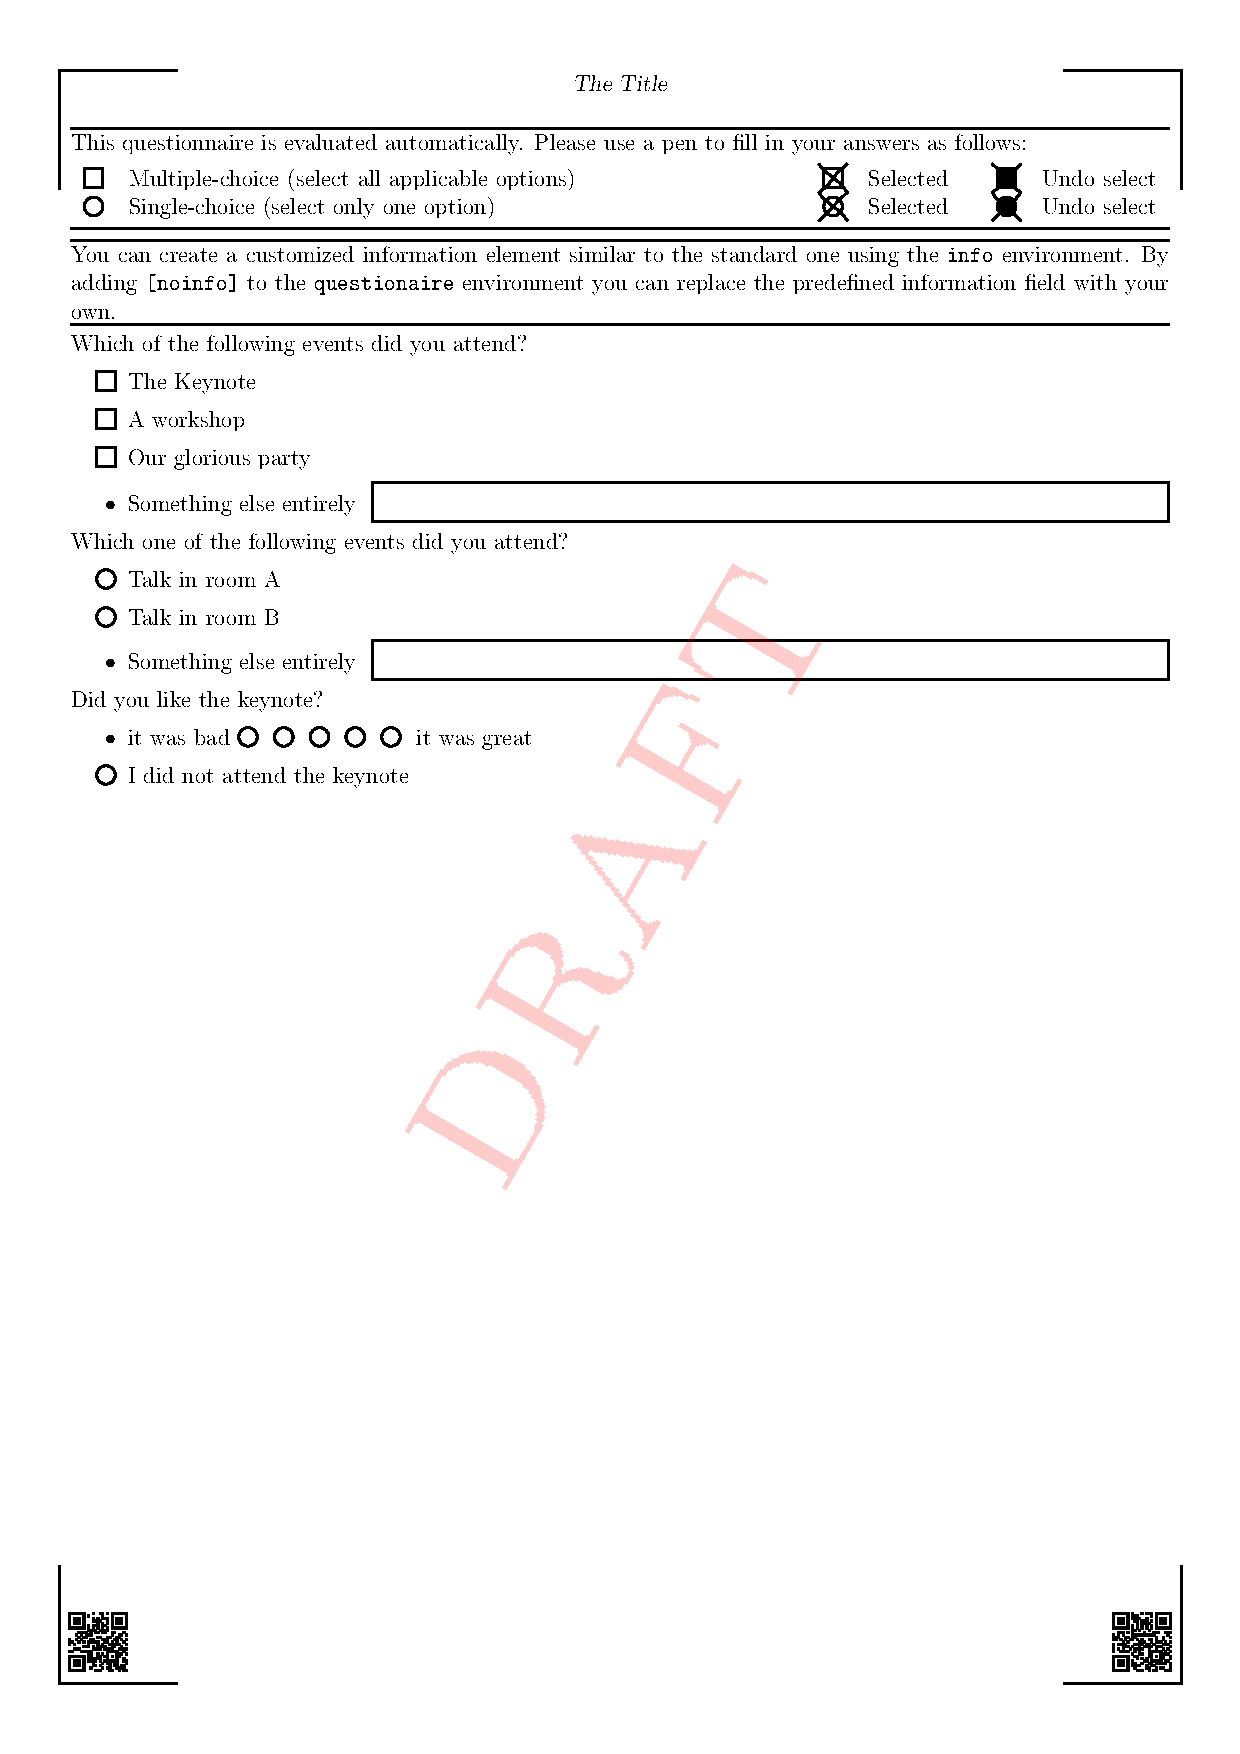
\includegraphics[scale=0.62]{600-Appendices/Questionnaire/Questionnaire}
		}
		\caption{Questionnaire to survey something}
	\end{figure}

\clearpage  % have next section on separate page
\section*{Appendix IV: Some \LaTeX{} examples}

This section is to be deleted/commented by the author.
\paragraph{Demonstration of abbreviations}
Define a glossary entry in file \textit{Acronyms.tex}:
\newline
\verb!\newacronym{utc}{UTC}{Coordinated Universal Time}!
\newline
Use a glossary entry: \verb! \gls{utc} !
\newline
This \LaTeX code \\

\verb*|\gls{utc} is 3 hours behind \gls{adt}.| \\

will produce this: \\

\gls{utc} is 3 hours behind \gls{adt}.\\

At the first time usage, the abbreviation is mentioned in brackets.

With the second usage of an abbreviation, the abbreviated term itself is not shown any more:
\gls{utc} is still 3 hours behind \gls{adt}.\\

\paragraph{Demonstration of a horizontal bar chart}
Fig. \ref{fig:XBarChart} shows an example of a horizontal bar chart generated with tikzpicture (pgfplots package).

\begin{figure}[!h]
	\centering
	\begin{tikzpicture}
		\begin{axis}[xbar,tick align=outside,
			%width=11cm,
			%height=8cm,
			bar width={10pt},
			enlarge y limits=0.13,
			enlarge x limits=false,
			nodes near coords,
			nodes near coords align=horizontal,
			use units,
			xmin=0,
			xmax=60,
			xtick={0,10,...,60},
			x unit=\%,
			xlabel=Reduction in diarrhoea morbidity,
			ytick={1,...,6},
			yticklabels={Hand Washing With Soap, Point-of-use Water Treatment, Sanitation, Hygiene Education, Water Supply, Source Water Treatment}
			]
			\addplot
			[draw=blue,fill=blue!15]
			coordinates
			{(11,1) (25,2) (28,3) (32,4) (39,5) (44,6)};
		\end{axis}
	\end{tikzpicture}
	\caption{\label{fig:XBarChart}Title to a x-bar chart}
\end{figure}

\paragraph{Demonstration of a vertical bar chart}
Fig. \ref{fig:YBarChart} shows an example of a vertical bar chart generated with tikzpicture (pgfplots package).


\begin{figure}
	\centering
	\begin{tikzpicture}
		\begin{axis}[ybar,tick align=outside,
			%width=11cm,
			%height=8cm,
			bar width={10pt},
			enlarge x limits=0.13,
			enlarge y limits=false,
			nodes near coords,
			nodes near coords align=vertical,
			use units,
			ymin=0,
			ymax=100,
			ytick={0,10,...,100},
			y unit=\%,
			ylabel=Response,
			xtick={1,...,7},
			xticklabels={Water for handwashing, Soap for handwashing, Covered pit latrines, Latrines condusive for use, Latrine have doors, Seperate for both boys and girls, Seperate for teachers/pupils},
			x tick label style={rotate=45,anchor=east}
			]
			\addplot
			[draw=blue,fill=blue!15]
			coordinates
			{(1,25) (2,10) (3,5) (4,45) (5,25) (6,100) (7,100)};
		\end{axis}
	\end{tikzpicture}
	\caption{\label{fig:YBarChart}Title to a y-bar chart}
\end{figure}

\paragraph{Demonstration of a stacked bar chart}
Fig. \ref{fig:StackedBarChart} shows an example of a stacked bar chart generated with tikzpicture (pgfplots package).

\begin{figure}
	\centering
	\begin{tikzpicture}
		\begin{axis}[ybar stacked, 
			xlabel=X achsis label, 
			ylabel=Y achsis label,
			legend cell align=left,
			legend pos=outer north east]
			\addplot coordinates 
			{(0,1) (1,1) (2,3) (3,2) (4,1.5)};
			\addplot coordinates
			{(0,1) (1,1) (2,3) (3,2) (4,1.5)};
			\addplot coordinates
			{(0,1) (1,1) (2,3) (3,2) (4,1.5)};
			\legend{Series 1, Series 2, Series 3}
		\end{axis}
	\end{tikzpicture}
	\caption{\label{fig:StackedBarChart}Title to a stacked bar chart}
\end{figure}

\paragraph{Demonstration of a clustered bar chart}
Fig. \ref{fig:ClusteredBarChart} shows an example of a clustered bar chart generated with tikzpicture (pgfplots package).

\begin{figure}
	\centering
	\begin{tikzpicture}
		\begin{axis}  
			[  
			ybar,
			ylabel={Y achsis label}, % there should be no line gap between the rows here. Otherwise, latex will show an error.  
			symbolic x coords={Dry, Rainy},  
			xtick=data,  % groups plots around same tick
			enlarge x limits=0.35, % increases the axis range by 25%
			ymin=0,
			major x tick style = transparent,
			nodes near coords,  
			nodes near coords align={vertical},
			legend cell align=left,
			legend pos=outer north east
			]  
			\addplot coordinates {(Dry, 75) (Rainy, 78)}; % these are the measures of a particular bar graph. The tick marks of the y-axis will be adjusted automatically according to the data values entered in the coordinates.  
			\addplot coordinates {(Dry, 70) (Rainy, 63)};  
			\addplot coordinates {(Dry, 61) (Rainy, 55)};  
			\legend{This, That, Other}  
			
		\end{axis} 
	\end{tikzpicture}
	\caption{\label{fig:ClusteredBarChart}Title to a clustered bar chart}
\end{figure}

\paragraph{Demonstration of a pie chart}
Fig. \ref{fig:PieChart} shows an example of a pie chart generated with tikzpicture (pgf-pie package).

\begin{figure}
	\centering
	\begin{tikzpicture}
		\pie [rotate = 180]
		{
			62/Category A,
			32/Category B, 
			6/Other
		}
		\end{tikzpicture}
	\caption{\label{fig:PieChart}Title to the pie chart}
\end{figure}

\paragraph{Demonstration of a line chart}
Fig. \ref{fig:LineChart} shows an example of a simple chart generated with tikzpicture (packages pgfplots and pgfplotstable). 
The regression is also rendered and the formula $ y(x_i) = a \cdot x_i + b$ displayed. The values a and b will be stored globally.

\begin{figure}
	\centering
	\begin{tikzpicture}
		\begin{axis}[legend pos=outer north east]
			\addplot table[row sep=\\] {% plot X versus Y. This is original data.
				X Y\\
				1 1 \\
				2 4\\
				3 9\\
				4 16\\
				5 25\\
				6 36\\
			};
			\addplot table[row sep=\\,
			y={create col/linear regression={y=Y}}] % compute a linear regression from the input table
			{
				X Y\\
				1 1 \\
				2 4\\
				3 9\\
				4 16\\
				5 25\\
				6 36\\
			};
			\addlegendentry{$y(x)$}
			\addlegendentry{%
				$\pgfmathprintnumber{\pgfplotstableregressiona} \cdot x
				\pgfmathprintnumber[print sign]{\pgfplotstableregressionb}$}
		\end{axis}

	\end{tikzpicture}
	\caption{\label{fig:LineChart}Title to the line chart}
\end{figure}

\paragraph{Demonstration of a table}
Table \ref{tbl:Salinity-EC} shows an example of a table. Different parts of the Final Year Report and their corresponding weights for marking them can be viewed at table \ref{tbl:ModuleWeight}.\\
A help to generate LaTeX tables can be found at \url{https://www.tablesgenerator.com/}.
\begin{table}
	\begin{center}
		\caption{\label{tbl:Salinity-EC}Conductivity values measured for defined salinity values}
		\begin{tabular}{cc}
			\hline \\
			Salinity [g/L]	& 	Electrical Conductivity [mS/cm]\\    
			\\
			\hline \\
			40	&	63,3	\\
			35	&	55,1	\\
			30	&	47,2	\\
			25	&	40,4	\\
			20	&	32,9	\\
			15	&	25,5	\\
			10	&	17,53	\\
			5	&	9,39	\\
			\hline \\
		\end{tabular}  
	\end{center}
\end{table}

\begin{table}
	\begin{center}
		\caption{\label{tbl:ModuleWeight}Module CIV4202 Final Year Report - Assessment}
		\begin{tabular}{llc}
			\hline \\
			Category					& Chapter or Feature				& Weight \\
			\\
			\hline \\
			Engineering Content (60\%)	& Introduction and Objectives		& 10\%   \\
										& Problem definition				& 5\%    \\
										& Literature review					& 5\%    \\
										& Methods							& 15\%   \\
										& Results and Discussion			& 15\%   \\
										& Conclusions and recommendations	& 10\%   \\
			Language (25\%)				& Grammar and spelling				& 15\%   \\
										& Sentence structure				& 10\%   \\
			References (15\%)			& Use of references					& 10\%   \\
										& Quality and format of references	& 5\%    \\
			\hline \\
		\end{tabular}
	\end{center}
\end{table}

\paragraph{Demonstration of including a PDF}
Fig. \ref{fig:GF543kv} shows an example of a PDF. The section displayed is of a particular page from the PDF and is cropped in size.
\begin{figure}
	\centering
	\includegraphics[height=0.7\textwidth,page=6, trim = 25mm 172mm 25mm 45mm, clip]{600-Appendices/Examples/Datasheet_GF_543}
	\caption{GF ball valve 543 kv-characteristic}
	\label{fig:GF543kv}
\end{figure}

\paragraph{Demonstration of including a graphics}
Fig. \ref{fig:ndulogo} shows an image stored as jpg-file. The file is limited to the page width and is rotated by 90\textdegree. Because of the rotation 'height' becomes 'width'.

\begin{figure}
	\centering
	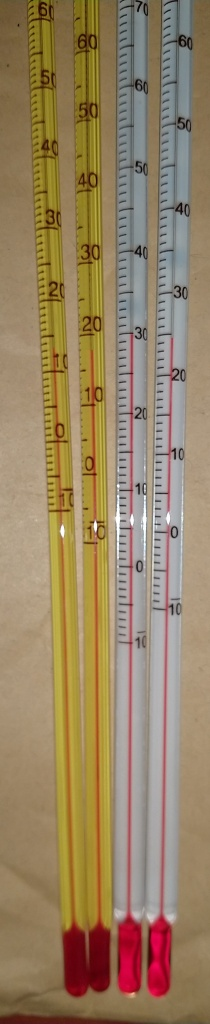
\includegraphics[height=1\textwidth, angle=90]{600-Appendices/Examples/Thermometer.jpg}
	\caption{Thermometers showing different temperature readings.}
	\label{fig:ndulogo}
\end{figure}

\paragraph{Demonstration of including a JPG with labels}
Fig. \ref{fig:HeatExchanger} shows an example of a JPG that has some labels applied.

\begin{figure}
	\centering
	\setlength {\unitlength}{0.1\textwidth}
	\begin{picture} (10,7)(0,0)
		\setlength\fboxsep{1 mm}
		\put(0,0){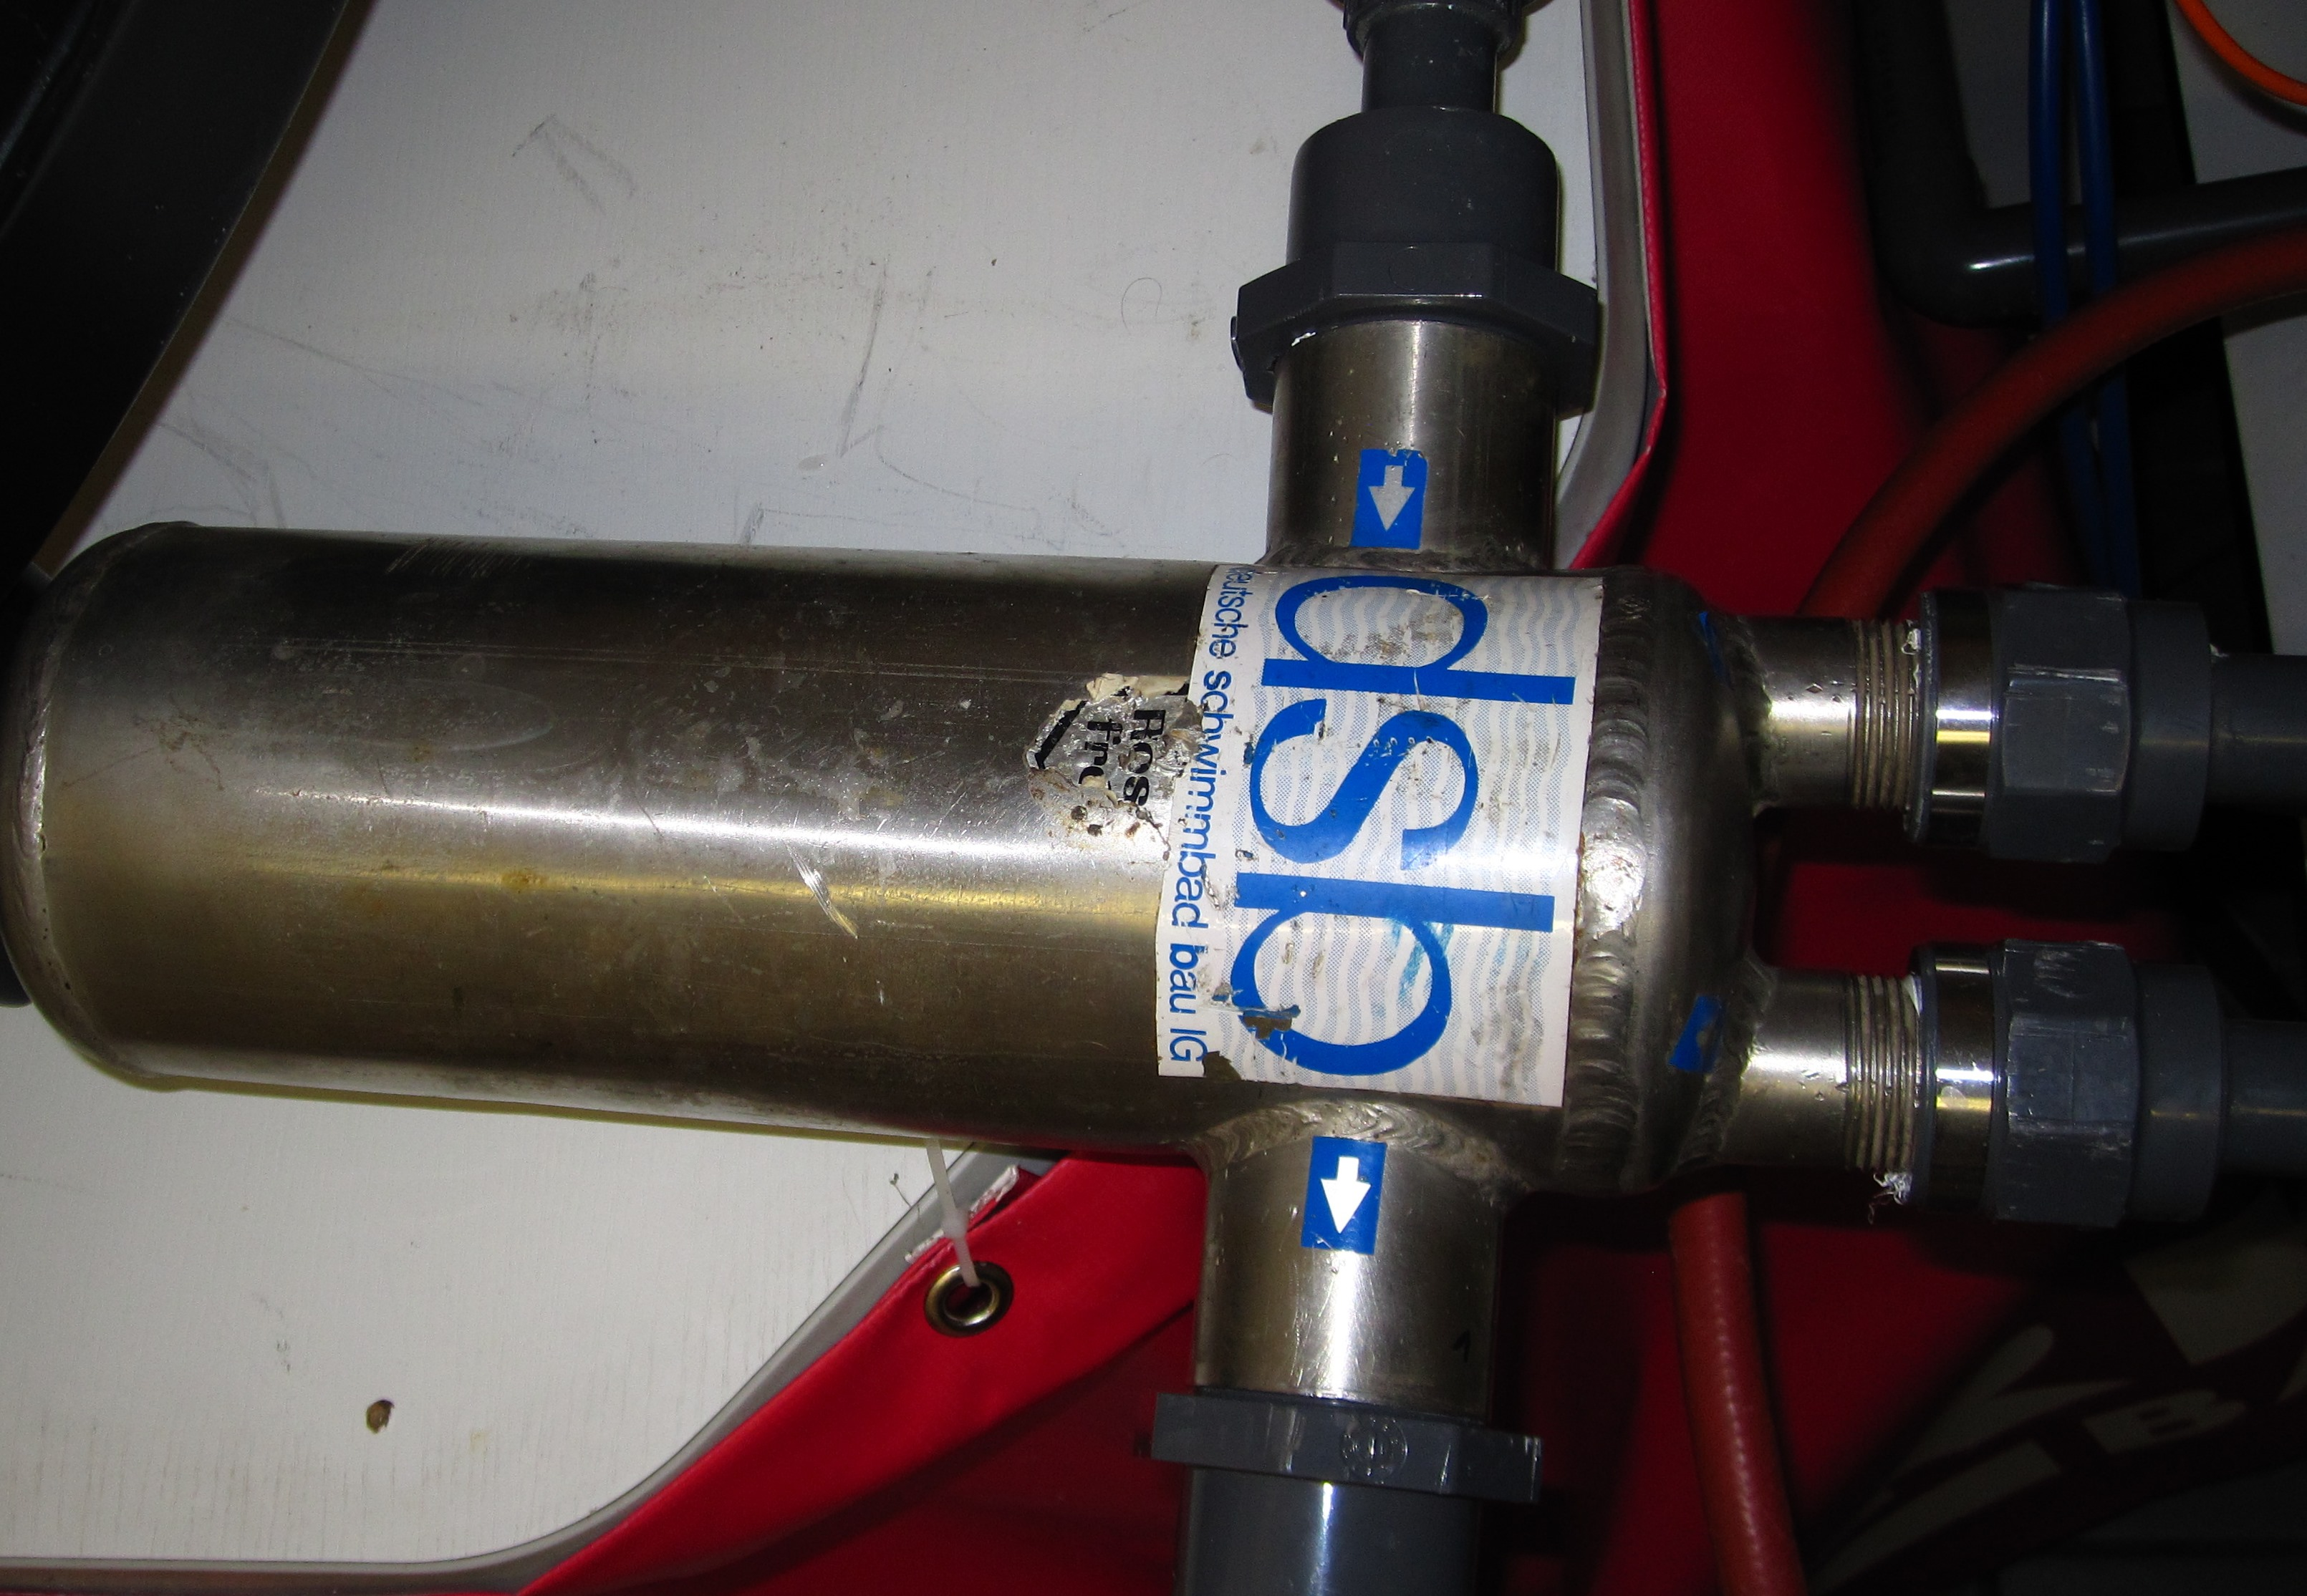
\includegraphics[width=\textwidth]{600-Appendices/Examples/Heat_Exchanger.jpg}}
		\put(4,5){\colorbox{red!20}{\framebox[1.1\width]{Concentrate in}}}
		\put(3,1){\colorbox{red!20}{\framebox[1.1\width]{Concentrate out}}}
		\put(7,4.5){\colorbox{blue!20}{\framebox[1.1\width]{From exchanger}}}
		\put(7,1.5){\colorbox{blue!20}{\framebox[1.1\width]{To exchanger}}}
	\end{picture}              
	\caption{Heat exchanger with flow of media}
	\label{fig:HeatExchanger}
\end{figure}

\paragraph{Demonstration of citation}
Table \ref{tbl:CitationStyles} shows some different options on how to cite a source. The examples are done using natbib package.

\begin{table}
	\begin{center}
		\caption{\label{tbl:CitationStyles}Some styles to citation}
		\begin{tabular}{lll}
			\hline \\
			Command & 	Output	& Description \\
			\\
			\hline \\
			\verb! \cite{ref} ! & \cite{Monippally2010} & Citation\\
			\verb! \textcite[page]{ref} ! & \textcite[p. 20]{Monippally2010} & Textual citation\\
			\verb! \parencite[chapter]{ref} ! & \parencite[chap. 4]{Monippally2010} & Parenthetical citation\\
			
			\verb! \citeauthor{ref} ! & \citeauthor{Monippally2010} & Name of author\\
			\verb! \citeyear{ref} ! & \citeyear{Monippally2010} & Year of publication\\
			\hline \\
		\end{tabular}  
	\end{center}
\end{table}

\cite{HowWriteDissertation} gives some guidance on how to structure a dissertation.

\paragraph{Demonstration of formulas}
Equation \eqref{equ:Population} shows the geometrical projection formula for population growth.
The parameters description is done using the macro \textit{conditions}, defined at NDUmacros.tex.

\begin{figure} % figure is used here to keep the block together
\begin{equation}\label{equ:Population}
P_f=P_0(1+\frac{i}{100})^t
\end{equation}
where:
\begin{conditions}
	P_f	&	Future population \\
	P_0	&	Current population \\
	i	&	Growth rate in \% \\   
	t	&	Time in years
\end{conditions}
\end{figure}

The Hazen-Williams formula expressed in metric units as seen in \eqref{equ:Hazen-William}.
\begin{figure} % figure is used here to keep the block together
\begin{equation}\label{equ:Hazen-William}
H[m]= \Big( \frac{6.78 L}{d^{1.165}} \Big) \Big({\frac{V}{C}} \Big)^{1.85}
\end{equation}
where:
\begin{conditions}
	H	&	Headloss \\
	L	&	Length of pipe\\
	d	&	Internal diameter of pipe \\   
	V	&	Flow \\
	C	&	Coefficient
\end{conditions}
\end{figure}
\paragraph{Demonstration of links}
Use \verb!\href{URL}{DESCRIPTION}! to add a link with description.
Use \verb!\url{URL}! to add a link without a description.

The Water Research \& Development Centre's website: \url{https://nduwrdc.org}

\paragraph{Demonstration of symbols}
In TeXstudio instead of viewing the \textit{Structure} in the side panel, click on $\ast$ to get a list of symbols. Once inserted a leading and trailing \$ must be placed around the symbol code. Some examples displayed using tabbing:
\begin{tabbing}
	\hspace{2in}     			\= \hspace{0.40in}  \= \hspace{1in}    		\kill
	\verb!$\pm$! 				\> $\rightarrow$ 	\> $\pm$ 				\\
	\verb!$\Longrightarrow$! 	\> $\rightarrow$ 	\> $\Longrightarrow$ 	\\
	\verb!$\alpha$! 			\> $\rightarrow$ 	\> $\alpha$ 			\\
	\verb!$\pi$! 				\> $\rightarrow$ 	\> $\pi$ 				\\
	\verb!$\mu$! 				\> $\rightarrow$ 	\> $\mu$	 			\\
\end{tabbing}

\paragraph{Demonstration of a flowchart}
You can follow the instructions of overleaf.com on creating flowcharts,  \url{https://www.overleaf.com/learn/latex/LaTeX\_Graphics\_using\_TikZ:\_A\_Tutorial\_for\_Beginners\_(Part\_3)\%E2\%80\%94Creating\_Flowcharts}, to achieve figures~\ref{fig:flowchart1}~and~\ref{fig:flowchart2}.
\begin{figure}
	\centering
	\begin{tikzpicture}[node distance=2cm]
		\node (start) [startstop] {Something to start with};
		\node (proc1) [process, right of=start, xshift=4cm] {Something else};
		\node (proc2) [process, below of=proc1, yshift=-0.5cm] {
			\begin{minipage}{4cm} %use minipage to have lists
				\begin{itemize}
					\item first item
					\item second item
				\end{itemize}
			\end{minipage}
			};
		\node (proc3) [process, below of=start, yshift=-.5cm] {more here};
		\node (proc4) [process, below of=proc3, xshift=2.5cm, yshift=-0.5cm,  align=left] {many lines\\line 2\\line 3\\line 4}; % align-key needed for \\linebreak 
		\draw [arrow] (start) -- (proc1);
		\draw [arrow] (start) -- (proc3);
		\draw [arrow] (proc1) -- (proc2);
		\draw [arrow] (proc3) -- (proc4);
		\draw [arrow] (proc4) -- (proc2);
	\end{tikzpicture}	
	\caption{Example of a flow chart}
	\label{fig:flowchart1}
\end{figure}

\begin{figure}
	\centering
	\begin{tikzpicture}[node distance=4cm]
		\node (start) [startstop] {Something to start with};
		\node (proc1) [process, right of=start, xshift=0.5cm, yshift=2cm] {A};
		\node (proc2) [process, right of=start, xshift=0.5cm, yshift=-2cm] {B};
		\node (proc3) [process, right of=proc1, yshift=1cm, align=left] {A1\\A1a};
		\node (proc4) [process, right of=proc1, yshift=-1cm, align=left] {A2\\A2b};
		\node (proc5) [process, right of=proc2, yshift=1cm] {B1};
		\node (proc6) [process, right of=proc2, yshift=-1cm] {B2};
		\draw [arrow] (start) -- (proc1);
		\draw [arrow] (start) -- (proc2);
		\draw [arrow] (proc1) -- (proc3);
		\draw [arrow] (proc1) -- (proc4);
		\draw [arrow] (proc2) -- (proc5);
		\draw [arrow] (proc2) -- (proc6);
	\end{tikzpicture}	
	\caption{Some sort of a tree}
	\label{fig:flowchart2}
\end{figure}

\paragraph{Demonstration of a circular diagram}
There is a number of examples using the smartdiagram package here: \url{https://texample.net/tikz/examples/all/}. Figure~\ref{fig:flowchart3} is one of them.
\begin{figure}
	\centering
	\smartdiagram[circular diagram:clockwise]{ABC, DEF, GHI, JKL, MNO}
	\caption{Circular diagram}
	\label{fig:flowchart3}
\end{figure}
		%% Questionnaires, interview transcripts, detailed tables\end{document}   % No characters allowed after this line

\end{document}   % No characters allowed after this line